% Chapter Template

\chapter{Ensayos y resultados} % Main chapter title

\label{Chapter4} % Change X to a consecutive number; for referencing this chapter elsewhere, use \ref{ChapterX}

%----------------------------------------------------------------------------------------
%	CHAPTER 4
%----------------------------------------------------------------------------------------

En este capítulo se explica cómo se llevaron a cabo las pruebas de validación de hardware y software a las que fue sometido el dispositivo, los bancos de ensayos e instrumentos utilizados y los resultados obtenidos.

\section{Banco de ensayos}

%\ref{fig:setupEnsayos}

%\begin{figure}[H]
%\centering
%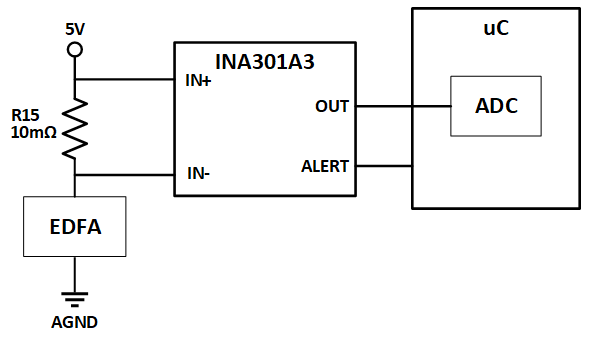
\includegraphics[width=0.75\textwidth]{./Figures/func_monitor.png}
%\caption{Esquema del monitor de corriente}
%\label{fig:setupEnsayos}
%\end{figure}

\section{Instrumental utilizado}

Para poder ejecutar las pruebas de integración de hardware y software del trabajo se requirió del uso de una variedad de instrumentos y equipos. La tabla \ref{tab:instrumentos} lista los detalles de cada uno de ellos.

\begin{table}[H]
	\centering
	\caption{Lista de instrumental utilizado.}
	\begin{tabular}{c c l}
		\toprule
		\textbf{Instrumento} & \textbf{Modelo} & \textbf{Descripción} \\
		\midrule
		Multímetro			&  UNI-T 				& asdasd \\
		Fuente 				& XXX					& XXXXX \\

		\bottomrule
		\hline
	\end{tabular}
	\label{tab:instrumentos}
\end{table}

\section{Pruebas de hardware}
\label{sec:pruebasHW}

% resistencias:
% alambre sobre tubo de ceramica, 25 ohm 50 W: AVT05006E25R00KE
% wirewound, 200 ohm 2 W: 3590S-1-201L

\subsection{Pruebas del monitor de corriente}



\subsection{Pruebas del monitor de tensión}



\subsection{Pruebas del relé de alimentación}



\section{Pruebas de software}
\label{sec:pruebasSW}



\subsection{Pruebas de la pantalla LCD}

